\documentclass[tikz,border=5pt]{standalone}
\usepackage{tikz}
\usetikzlibrary{calc}
\begin{document}
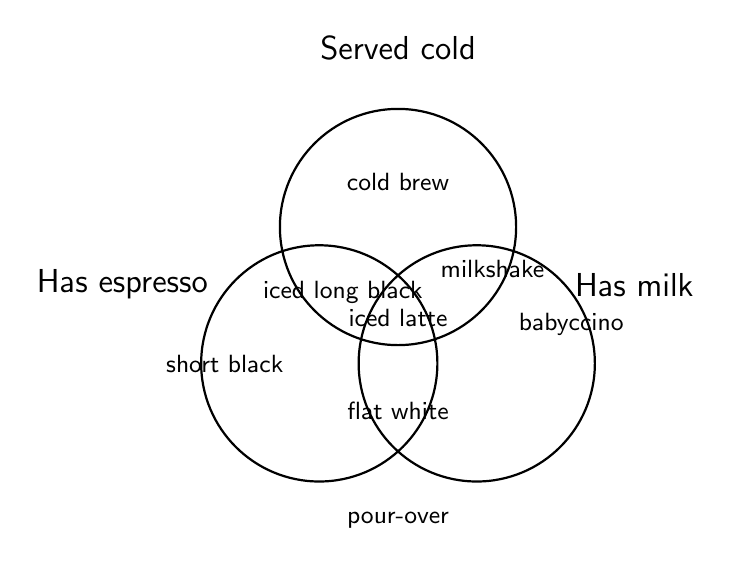
\begin{tikzpicture}[scale=1.0, every node/.style={font=\sffamily}]
% Circle parameters
\def\radius{1.5}
\coordinate (A) at (0,0);   % Has espresso
\coordinate (B) at (2,0);   % Has milk
\coordinate (C) at (1,{sqrt(3)}); % Served cold

% Draw circles
\draw[thick] (A) circle (\radius);
\draw[thick] (B) circle (\radius);
\draw[thick] (C) circle (\radius);

% Circle labels (outside circles)
\node at (-2.5, 1) {\large Has espresso};
\node at (4, 1) {\large Has milk};
\node at (1, 4) {\large Served cold};

% Drink names in appropriate regions
% Outside all circles
\node at (1,-2) {\small pour-over};

% A only (espresso only)
\node at (-1.2,0) {\small short black};

% B only (milk only)
\node at (3.2,0.5) {\small babyccino};

% C only (cold only)
\node at (1,2.3) {\small cold brew};

% A∩B only (espresso + milk)
\node at (1,-0.6) {\small flat white};

% A∩C only (espresso + cold)
\node at (0.3,0.9) {\small iced long black};

% B∩C only (milk + cold)
\node at (2.2,1.2) {\small milkshake};

% A∩B∩C (espresso + milk + cold)
\node at (1,{sqrt(3)/3}) {\small iced latte};
\end{tikzpicture}
\end{document}